\documentclass[../portafolio.tex]{subfiles}

% Solo agregue paquetes en el preámbulo de ../portafolio.tex

\begin{document}

% En esta sección, explique en detalle los siguientes aspectos:
% - Fecha de realización de la actividad
% - Título de la actividad (dentro de \section)
% - Un párrafo explicando cuál es el objetivo de la actividad
% - Nombre de personas con quien trabajó en la actividad
% - Una selección de evidencias de que usted hizo esta actividad (imágenes, códigos, respuestas a un problema teórico, etc.)
% - Una conclusión breve (qué aprendió con la actividad, qué no entendió, qué faltó trabajar, qué recomienda para futuras sesiones)

% Numero máximo de palabras en esta sección: 1000 palabras.

%%%%%%%%%%%%%%%%%%%%%%%%%%%%%%%%%%%%%%%%%%%%%%%%%%%%%%%%%%%%%%%%%%%%%%%%%%%%%%%%
\section{Título de la actividad}   % ejemplo: Derivadas numéricas , introducción a git , 

\hfill \textbf{Fecha de la actividad:} 19 de agosto de 2022

\medskip

%---------------------------------------------------------------------------------
% Introducción/objetivos de la actividad
Escriba un párrafo explicando cuáles son los objetivos de la actividad.

%---------------------------------------------------------------------------------
% Con quién hizo esta actividad
Escriba un párrafo simple indicando si hizo la actividad
individualmente o en grupo. Si lo hizo en grupo, indique los nombres
de las personas con quien trabajó.


%---------------------------------------------------------------------------------
% Selección de evidencias

Explique detalladamente las evidencias de que usted realizó la actividad. Para esto, puede utilizar ecuaciones dentro
del texto como $\frac{x}{\sqrt{1-x^2}}$, o bien ecuaciones enumeradas,
por ejemplo:
\begin{equation}\label{eq:euler}
\exp(i\theta) = \cos(\theta) + i\sin(\theta).
\end{equation}

Puede citar ecuaciones enumeradas, por ejemplo la ecuación
\eqref{eq:euler} es una de las ecuaciones básicas del cálculo
complejo.

También puede agregar figuras para explicar mejor sus ideas. Trate de
citarlas adecuadamente en el texto, por ejemplo, la figura
\ref{fig:estatica} muestra un ejemplo usado en wikipedia
para explicar la electricidad estática~\cite{wikistatic}.

\begin{figure}[h!]
  \centering
  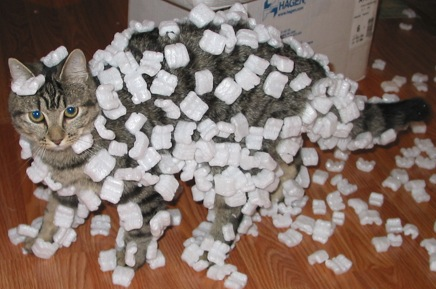
\includegraphics[width=0.5\textwidth]{static_cat_wikipedia.jpg}
  \caption{Bolas de poliestireno adheridos al pelaje de un gato debido
    a la electricidad estática.~\cite{wikistatic}.}
  \label{fig:estatica}
\end{figure}


\subsection{Una subsección}

Si cree necesario, puede separar el texto en subsecciones.



\end{document}
